\pagenumbering{gobble}
\documentclass{slides}
\usepackage{times}



\usepackage{amsmath,amsthm,amssymb,color}
%\usepackage{multicol}
\usepackage{graphicx}
\usepackage{fullpage}
\usepackage{hyperref}
%\usepackage{courier}
\usepackage{listings}
\usepackage{color}
%\usepackage[all]{hypcap}

\newcommand{\Squash}{\mathsf{Squash}}
\newcommand{\Clamp}{\mathsf{Clamp}}
\newcommand{\Range}{\mathsf{Range}}

\let\x\cdot
\lstset{
  language=Python,
  showstringspaces=false,
  tabsize=4,
  basicstyle=\ttfamily,
  keywordstyle=\bfseries\ttfamily,
  captionpos=b
}
\lstdefinelanguage{JavaScript}{
  keywords={if,else,var},
  keywordstyle=\bfseries\ttfamily,
  sensitive=false,
  comment=[l]{//},
  morecomment=[s]{/*}{*/}
}


\begin{document}

\title{\bf Range Analysis for the IonMonkey JavaScript Compiler}
\author{Ryan Pearl and Michael Sullivan}

\maketitle

\begin{slide}
\begin{center}
{\Huge \bf{IonMonkey}}
\end{center}

\begin{itemize}
\item IonMonkey is Mozilla's next generation Javascript engine
\item Optimizing JIT compiler
\item Modern SSA-based compiler with internals inspired by LLVM
\item Performs optimistic type specialization and bails out when type
  assumptions fail
\item Designed to be easy to extend
\end{itemize}
\end{slide}

\begin{slide}
\begin{center}
{\Huge \bf{JavaScript Arithmetic}}
\end{center}
\begin{itemize}
\item JavaScript numbers defined to be double precision floating point
\item For efficiency, implementations store and operate on them as
  integers whenever possible
\item IonMonkey will generates type specialized code for integer values
\item If arithmetic overflows, need to bail out of integer code and
  promote to doubles
\item Range analysis could eliminate these overflow checks
\end{itemize}
\end{slide}

\begin{slide}
\begin{center}
{\Huge \bf{Range Analysis}}
\end{center}
\begin{itemize}
\item Associate each integer temporary with a range: a contiguous subset of $\{-\infty\} \cup [-2^{31}, 2^{31}-1] \cup \{\infty\}$
\item Infinite ranges indicate the operation can overflow; arithmetic operations with a finite range don't need overflow checks!
\item Can do arithmetic on ranges:
\end{itemize}
\begin{eqnarray*}
\Clamp(n) &=& \begin{cases}
-\infty &\text{if } n < -2^{31} \\
\infty &\text{if } n > -2^{31}-1 \\
n&\text{otherwise } \\
\end{cases}\\
\Clamp([l, h]) &=& [\Clamp(l), \Clamp(h)] \\
{[x_l, x_h] \cup [y_l, y_h]} &=& [\min(x_l, y_l), \max(x_h, y_h)] \\
{[x_l, x_h] \cap [y_l, y_h]} &=& [\max(x_l, y_l), \min(x_h, y_h)] \\
{[x_l, x_h] + [y_l, y_h]} &=& \Clamp ([x_l + y_l, x_h + y_h]) \\
{[x_l, x_h] - [y_l, y_h]} &=& \Clamp ([x_l - y_h, x_h - y_l])
\end{eqnarray*}
\end{slide}


\begin{slide}
\begin{center}
{\Huge \bf{XSA Form}}
\end{center}
\begin{itemize}
\item Want a way to track information learned from conditionals without needing to consider more than one range per temp
\item Introduce $\beta$ nodes to associate range information from conditionals with temporaries
\item Some example code with $\beta$ nodes; all of the ranges checks can be eliminated
\end{itemize}
{\tiny
\begin{verbatim}
if (x < 0) {
    x1 = Beta(x, [INT_MIN, -1]);
    y1 = x1 + 2000000000;
} else {
    x2 = Beta(x, [0, INT_MAX]);
    if (x2 < 1000000000) {
        x3 = Beta(x2, [INT_MIN, 999999999]);
        y2 = x3*2;
    } else {
        x4 = Beta(x2, [1000000000, INT_MAX]);
        y3 = x4 - 3000000000;
    }
    y4 = Phi(y2, y3);
}
y = Phi(y1, y4);
\end{verbatim}
}
\end{slide}

\begin{slide}
\begin{center}
{\Huge \bf{Range Analysis Algorithm}}
\end{center}
\begin{itemize}
\item Range analysis is simple and worklist based. Range recomputation is done with range arithmetic. $\beta$ intersects a range, $\phi$ unions.
\item Key insight: can always squash inputs to a finite range, since they would have bailed out if they overflowed.
\end{itemize}
{\tiny
\begin{verbatim}
def propagateRanges(graph):
    worklist = []
    for block in reversePostOrder(graph):
        for insn in block:
            insn.recomputeRange()
            if !insn.isPhi() and !insn.isBeta():
                continue
            worklist.appendAll(insn.uses())

    while len(worklist) > 0:
        insn = worklist.pop()
        #recomputeRange() returns true if the range changed
        if (insn.recomputeRange()):
            worklist.appendAll(insn.uses())
\end{verbatim}
}
\end{slide}

\begin{slide}
\begin{center}
{\Huge \bf{Results}}
\end{center}
\begin{itemize}
\item Instrumented IonMonkey to output percentage of adds and
  subtracts eliminated on a number of standard benchmark tests
\item Encouraging results
\end{itemize}
\centering
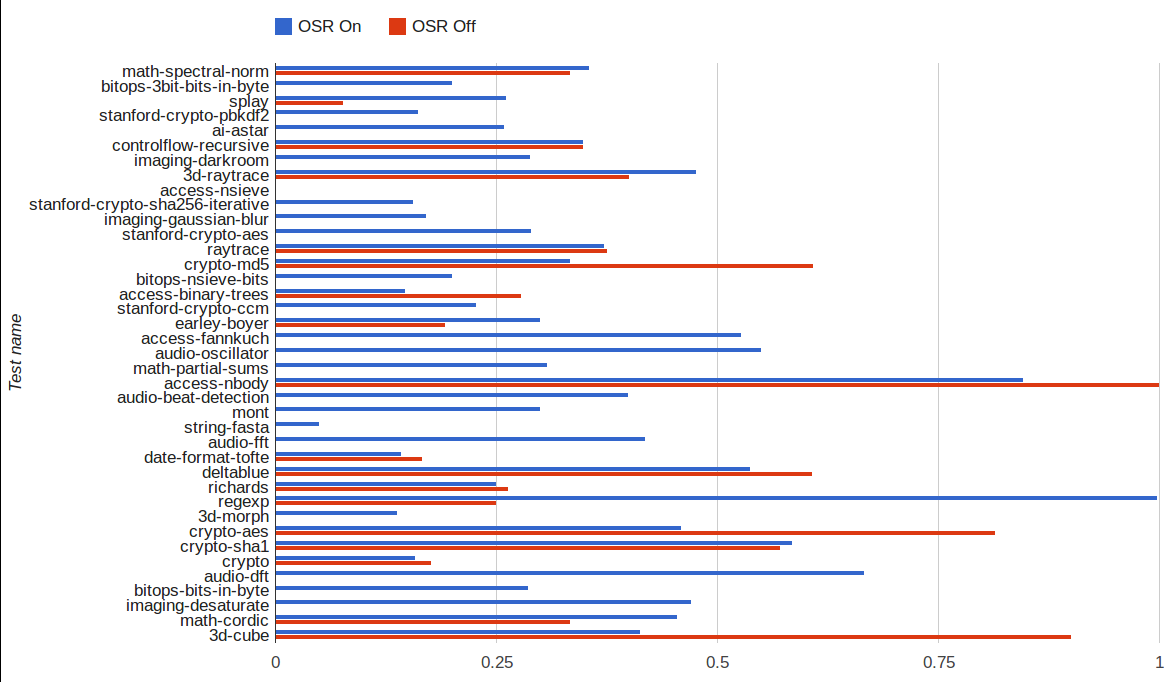
\includegraphics[width=0.98\textwidth]{counts_graph.png}
\end{slide}


\begin{slide}
\begin{center}
{\Huge \bf{Results }}
\end{center}
\begin{itemize}
\item Tested with three benchmark suites: v8bench, Sunspider, and Kraken
\item No statistically significant effect on v8bench
\item Tiny performance regression on Sunspider (0.1\%)
\item 1.5\% performance improvement on Kraken
\item Real overall wins, but not much.
\item Branch prediction is good these days, overflow checks wind up as
  noise in real programs
\item Microbenchmarks can see 30\% improvement
\end{itemize}
\end{slide}


\end{document}
